%----------------------------------------------------------------------------
\chapter{\pojo}
\label{sec:pojochapter}

Ebben a fejezetben bemutatom a {\thetaSc} reprezentációt. Mivel egy már korábban mások által elkezdett projektet fejeztem be külön kitérek arra is, hogy mely részek a saját fejlesztésem részei.
%----------------------------------------------------------------------------
\section{Az állapotgép}
%----------------------------------------------------------------------------
Az állapotgép egy széles körben használt modellezési módszer. A modellezni kívánt rendszerünket több egymástól jól elkülöníthető állapotokra bontjuk, ez lesz a rendszer állapota. Elvégezhetünk különféle feladatokat, akkor ha belépünk, vagy akkor ha kilépünk az adott állapotból.

\begin{figure} [!ht]
\centering
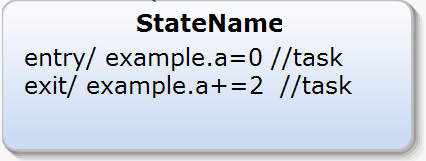
\includegraphics[width=60mm, keepaspectratio]{figures/state.png}
\caption{\label{fig:state}Egy állapot Yakinduban.}
\end{figure}

A rendszer természetesen működés közben változik, másik állapotba kerül. Az állapotváltást a tranzíciók segítségével írjuk le. Ezeket mindig valamilyen esemény váltja ki, lehet egy felhasználói esemény, vagy egy időzített esemény. Őrfeltételt is adhatunk \verb+[]+-en belül ilyenkor csak akkor lépünk át a másik állapotba, ha ez a feltétel teljesül. A \verb+/+ után pedig újabb parancsokat hajthatunk végre

\begin{figure} [!ht]
 	\centering
 	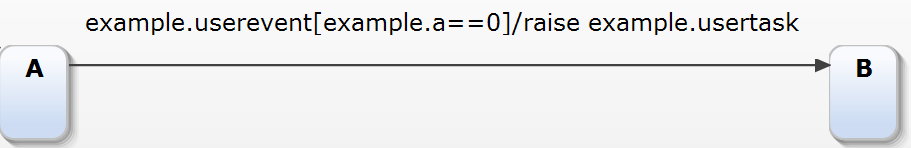
\includegraphics[width=150mm, keepaspectratio]{figures/transition.png}
 	\caption{\label{fig:transition}Egy tranzíció Yakinduban.}
\end{figure}

Előfordulhat az is, hogy több állapotot valamilyen közös tulajdonságuk szerint szeretnénk csoportosítani. Ilyenkor jók az összetett állapotok.\label{infovesztes} Ezt az információt veszítjük tehát el, ha "kilapítjuk"\footnote{Több állapot felvételével helyettesítjük az összetett állapotokat} az állapotgépet.

Itt kell bevezetni a régió fogalmát. Minden állapot egy régióban van, és minden régióban egyszerre csak egy állapot írhatja le a rendszerünket. Az összetett állapotok tehát tartalmaznak legalább egy régiót.

A régión belül van egy úgynevezett pszeudo állapot, ami kijelöli, hogy egy régióba lépés esetén melyik állapotba lépjünk. Három fajtája van a history, deephistory és a sima kezdő állapot. A sima mindig ugyanarra az állapotra mutat, a history megjegyzi, hogy kilépéskor melyik volt aktív és oda léptet vissza. A deephistory még ennél is többet jegyez meg, ha a kilépéskori aktív állapot, egy összetett állapot, akkor az azon belüli aktív állapotokat is megjegyzi.

\begin{figure} [!ht]
	\centering
	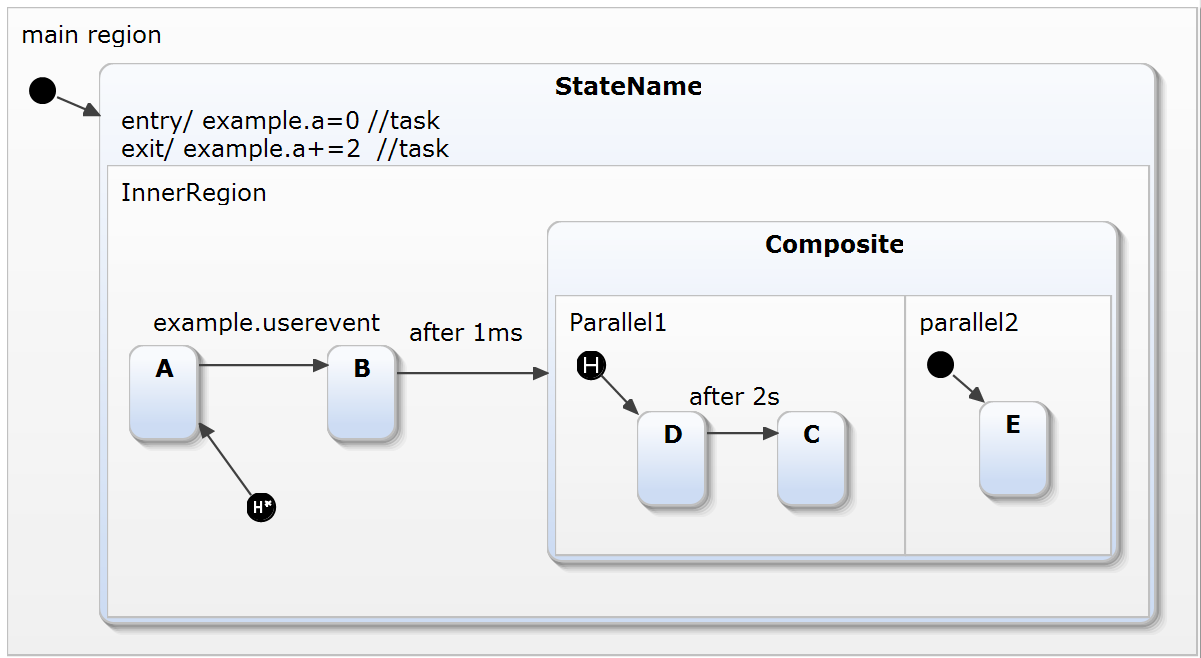
\includegraphics[width=150mm, keepaspectratio]{figures/statechart.png}
	\caption{\label{fig:statechart}Egy összetett állapotgép Yakinduban.}
\end{figure}


%----------------------------------------------------------------------------
\section{A {\thetaSc}}
\label{sec:thetaleiras}
%----------------------------------------------------------------------------

Az állapotgép reprezentáció Java-ban készült el. Az egyes osztályok megfeleltethetők az előző fejezetben leírt állapotgép elemekkel. Mindegyik osztálynak vannak a tárolt elemeihez getter/setter, a tárolóikhoz pedig add függvényei. Illetve néhány segédfüggvény, ami segít majd az analízis közben. A projekt már korábbi munkák folytatásaként jött létre. Az én hozzájárulásom a pszeudo állapotok implementálása, az időzített események kezelése és néhány segéd függvény, illetve apróbb javítások.


\begin{lstlisting}[language=java,breaklines=true]
interface Sc {}
\end{lstlisting}

Az állapotgépet reprezentáló interfész. Ez tárolja a gyökér régiót. Van neve, tárolja az összes tranzíciót az állapotgépben. Tárolja a változó deklarációkat egy a Thetában értelmezett osztályban (VarDecl). 

Az egyetlen megvalósító osztály a \verb+MutableSc+ minden tárolója hashSet-ben van megvalósítva

\begin{lstlisting}[language=java,breaklines=true]
interface Region {}
\end{lstlisting}

Van neve, tárolja az állapotait (State), ezek lekérdezhetőek és pontosan egy pszeudó állapota (PseudoState) van. Lehet szülő állapota; az állapot ami közvetlen őt tartalmazza. Továbbá van egy Boolean attribútuma, ami azt jelzi, hogy RootRegion-e a régió azaz nincs neki szülőállapota. Ellenőrizhető, hogy szabályos-e a régió: Minden tartalmazás igaz fordított irányban (vagyis az elem szülő eleme a régió)

Az egyetlen megvalósító osztály a \verb+MutableRegion+ egy hashSet-ben tárolja az állapotait

\begin{lstlisting}[language=java,breaklines=true]
interface State {}
\end{lstlisting}

Van neve és tárolja a régióit (Region) ez lehet egy üres lista. Kötelezően van szülő régiója. Van két akciója (Action), egy a kimeneti, egy a bemeneti akcióknak. Van két tranzíció tárolója, tárolja ugyanis a beérkező tranzíciókat és a kimenőket is.

Az egyetlen megvalósító osztály a \verb+MutableState+ minden tárolója hashSet-ben van megvalósítva

\begin{lstlisting}[language=java,breaklines=true]
interface Transition {}
\end{lstlisting}

A tranzíciót reprezentáló interfész. Tárolja a forrás állapotát (honnan indul ki) és a cél állapotát (hova érkezünk). Továbbá van egy kiváltó (trigger) eseménye (Event). Lehet őrfeltétele, ami a Thetában is használt Expr<Type> osztály. Van egy akciója (Action)

Az egyetlen megvalósító osztály a \verb+MutableTransition+

\begin{lstlisting}[language=java,breaklines=true]
interface PseudoState {}
\end{lstlisting}

Van neve, tárolja azt az egy állapotot ami a régiójába lépéskor az aktuális állapot lesz. Kötelezően kell legyen egy szülő régiója (Region).

Három megvalósító osztály a \verb+MutableInitState+ a sima kezdő ~ a \verb+MutableHistorytate+ a history~ a \verb+MutableDeepHistoryState+ pedig a deephistory pszeudo állapothoz

\begin{lstlisting}[language=java,breaklines=true]
interface Action {}
\end{lstlisting}

Interfész az akcióknak. Visitor mintát követi. Négy különböző osztály van. 

Az \verb+AssignmentAction+ egy egyszerű változó értékadást reprezentál, van tehát egy változója (VarDecl) és egy kifejezése (Expr).

A \verb+SignalAction+ egy esemény (Event) jelzést reprezentál. Ennek megfelelően tárol egy eseményt (csak egyet)

Az \verb+EmptyAction+ azért van, hogy ne null-okat tároljunk ha egy tranzíciónak, vagy állapotnak nincs akciója

A \verb+SequenceAction+ Több akciót (Action) tárol

\begin{lstlisting}[language=java,breaklines=true]
interface Event {}
\end{lstlisting}

Az eseményeket reprezentáló interfész alapvetően, csak egy neve van.

Két megvalósító osztály van az \verb+EventImpl+ a user eseményekhez, a \verb+TimeEventImpl+ pedig az időzített eseményeknek a \hyperref[fig:statechart]{3.3-as ábrán} is látható after 2s is egy ilyen esemény. Tárolja a nevén kívül azt, hogy mennyi az időzítés (milliszekundumban).


%----------------------------------------------------------------------------
\section{Sorosítás}
%----------------------------------------------------------------------------

Amikor egy adott modellen akarunk végezni analízist, valószínűleg nem csak egyszer tesszük ezt meg, hanem többször is. Nem lenne túl hatékony, ha mindig újra kéne építeni az állapotgépet, erre van a sorosítás, vagy szerializáció, ami lehetővé teszi az állapotgépek gyors beolvasását, illetve akár néhány módosítás utáni kiírását.

A séma Lisp-szerű szintaxist követ. A \hyperref[sec:thetaleiras]{fent} említett elemek sorosítva a következőképp néznek ki:

\begin{lstlisting}[language=java,breaklines=true]
(statechart nameOfStateChart
	(var varName varType)
	(var var2 type)
	(event Esemény)
	(region regionName
		(state stateName
			(entry assign varName value)
			(exit assign var2 value))
		(state compositeState
			(region innerRegion
				(state inState)
				(state stateA))
				(init inState))
		(history stateName))
	(transition stateName compositeState
		(trigger Esemény)
		(guard varName>2)
		(effect 
			(sequence
					(assign varName value)
					(signal Esemény))))
\end{lstlisting}

Azt érdemes megemlíteni, hogy egy-egy elemet előbb deklarálunk, például (var varName varType) és utána már elég a nevével hivatkozni rá. Például (assign varName value)

\begin{figure} [!ht]
	\centering
	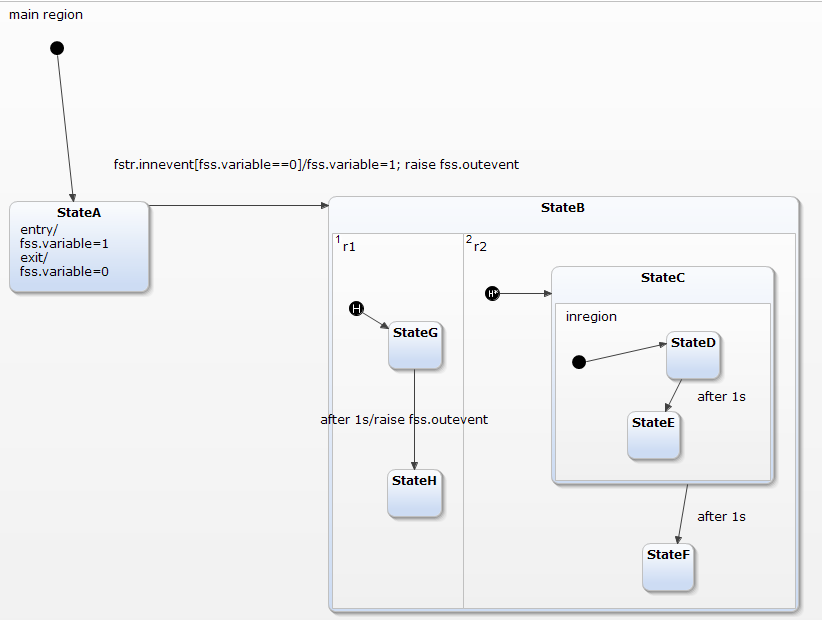
\includegraphics[width=150mm, keepaspectratio]{figures/serializeexample.png}
	\caption{\label{fig:serializeexample}példa állapotgép a szerializációhoz}
\end{figure}

\begin{figure} [!ht]
\centering
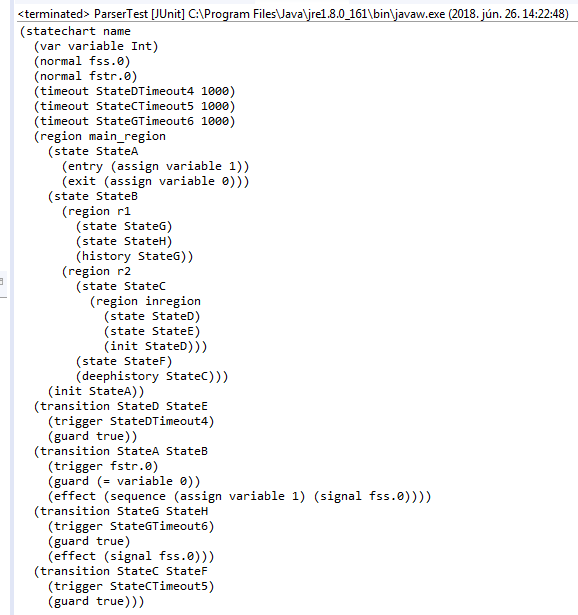
\includegraphics[width=150mm, keepaspectratio]{figures/serializeresult.png}
\caption{\label{fig:serializeresult}a \hyperref[fig:serializeexample]{fenti} állapotgép sorosítva}
\end{figure}

